\newpage
\section{Hardware}
\label{sec:hardware}
\hspace{\parindent}
As, much of the code behavior depends on the hardware it is used with, it is important to describe what hardware we had available in the development of TSEngine.
Due to the fact that TSEngine is a graphics engine adapted to the virtual reality, we have dealt with some unique devices, like head mounted displays and Cyberith treadmill, but the GPU's that we have tested the code on will also be described.
\begin{itemize}
    \item VR headsets:
    \begin{itemize}
        \item HTC VIVE Pro Full Kit x2\\
        This headset first introduced us to the concept of VR as it was available to the robotics club, and instantly inspired us to make the TSEngine. The VIVE Pro has a resolution of 2880 x 1600 pixels per eye, refresh rate of 90 Hz and 110 degrees of vision, allowing for great immersion and detailed vision. Its distinct feature is the use of lighthouse tracking system, which allows smooth motion tracking, and was the first headset that used HTC VIVE Base Station 2.0, which are now the standard for motion tracking used for example in Valve Index.
        \begin{figure}[H]
        \begin{center}
         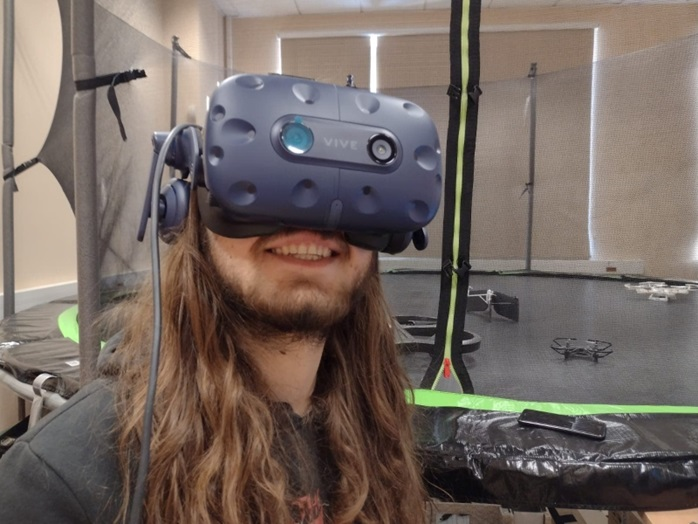
\includegraphics[width=0.7\textwidth]{vr_in_action_1.jpg}           
        \end{center}
         \caption{Headset in action}
        \end{figure}
        \item Oculus Quest 2\\
        Another headset that was used in the development of TSEngine was Oculus Quest 2. It is a newer headset compared to the VIVE one, released in 2020 compared to VIVE that was released in 2018, and as such has some clear advantages. First of all, it is a self-contained headset that does not require a PC or smartphone to operate, making it a more accessible option for VR gaming. Another advantage is its price, which is quite cheaper compared to VIVE Pro, allowing a wider audience to buy the headset, and propagate the idea of VR. As the headset itself contains all the necessary sensors to track its position and orientation, it doesn't need any additional devices like lighthouses to track the position of the headset and controllers. This approach is more affordable and portable, but sometimes works worse than using lighthouses. Oculus Quest 2 has a resolution of 1832 x 1920 pixels per eye, refresh rate of 90 Hz and 101 degrees of vision, which comes up to a great, easy to use and affordable VR headset.
    \end{itemize}
    \item Cyberith Virtualizer Elite 2\\
    In the making of TSEngine, it was suggested  that we used Cyberith Virtualizer Elite 2 as a means of motion input, as it was available to the robotics club. It is an interesting device, an omnidirectional treadmill developed to be used in pair with VR, and is further explained in section \hyperref[sec:virtualizer]{\ref*{sec:virtualizer}. Virtualizer}
    \begin{figure}[H]
    \begin{center}
     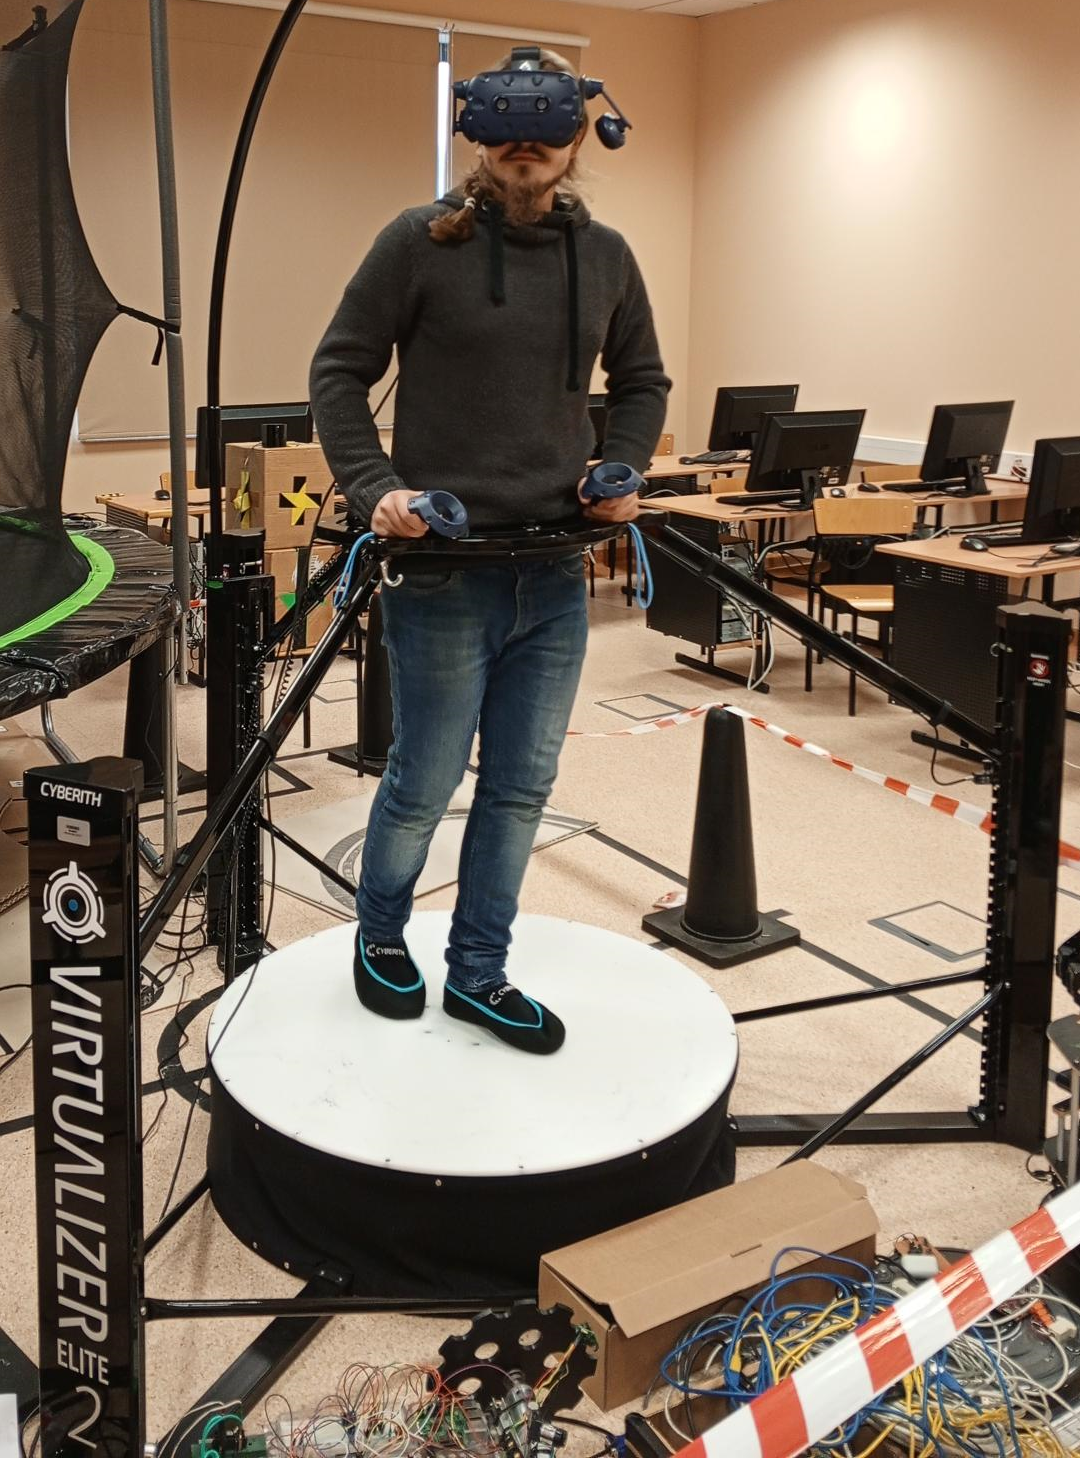
\includegraphics[width=0.55\textwidth]{figures/dominik.png}
    \end{center}
      \caption{Treadmill in action}
    \end{figure}
    \item GPUs:\\
    When working with computer graphics, one must consider that some features that work great for one GPU, can be problematic for another. Here are the GPU's TSEngine have been developed and tested on.
    \begin{itemize}
        \item NVIDIA RTX 3050\\
        \item NVIDIA RTX 2080\\
        \item NVIDIA RTX 2060\\
        \item NVIDIA GTX 1650\\
        \item AMD Radeon RX 7900 XT\\
    \end{itemize}
\end{itemize}
  

